\section{电子的发现}

19世纪末期, 关于真空管的实验很流行.
科学家们发现在真空管内加上电极和电压, 随着电压的增大,
会发生真空放电现象, 在真空管的阴极会发出阴极射线(cathode rays).
阴极射线是什么, 具体说是一种粒子,
还是一种波动(电磁波)就成了19世纪末期科学家们争论的一个热门问题。

\subsection{汤姆逊实验}

\begin{figure}[h]
\begin{center}
  % Requires \usepackage{graphicx}
  \includegraphics[width=5cm]{AtomIdea/perrin.ps}\\
  \caption{佩林实验}\label{Perrin experiment}
\end{center}
\end{figure}



1895 佩林通过用量电器(electrometer)收集阴极射线表明这种射线带负电,
实验如图(\ref{Perrin experiment}). 英国科学家们认为阴极射线是粒子,
而德国科学家们则倾向于波. 为了验证自己的想法, 1897
年英国科学家汤姆逊(Thomson)进行了实验.
汤姆逊认为阴极射线就是带电粒子流, 质量为$m$, 电荷为$e$,
通过测量阴极射线在外加电场(或磁场)真空管内的偏转,
汤姆逊测量了带电粒子的荷质比(specific charge),
这种粒子正是我们现在所说的“电子”(electron)。

\begin{figure}[h]
\begin{center}
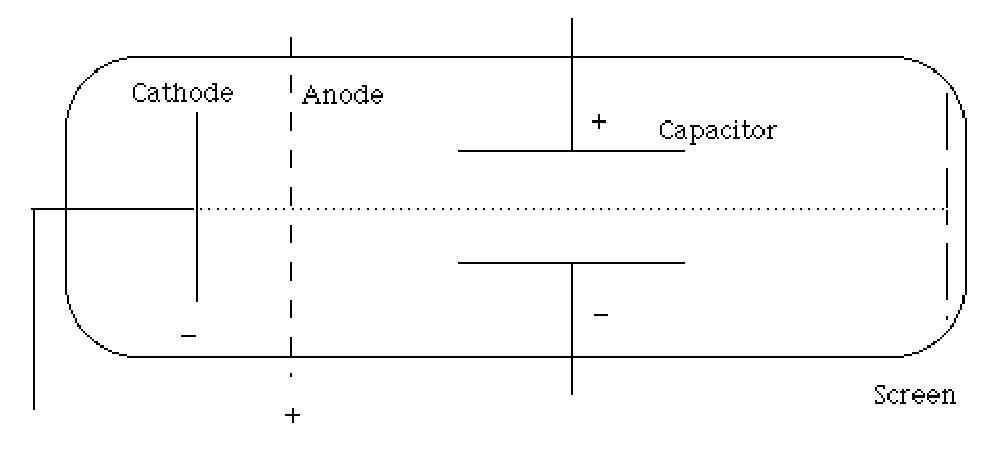
\includegraphics[clip,width=8cm]{AtomIdea/1-1.eps}
\caption{汤姆逊实验示意图}
\end{center}
\end{figure}

\begin{enumerate}
\item{首先,用阴极射线照射电量计,发现电量计逐渐积累了负电荷;(说明粒子流带负电)}

\item{在阴极射线管内加强磁场,发现阴极射线会弯曲;(带电粒子在磁场内可作圆周运动)}

\item{在电容器(capacitor)上加电压$V$,发现阴极射线会向上弯曲;}

\item{在垂直方向加合适的磁场B,可以使阴极射线重新回到原点,抵消因为加电场所引起的弯曲;}

\end{enumerate}

实验的第4个步骤说明运动粒子在磁场内所受洛仑兹力与库仑力正好抵消:$|ev
\times B| = |eE|$,可计算出粒子运动速度: $v =
E/B$。我们可以测量电场为零情况下,粒子运动半径r,$m\frac{{v^2 }}{r}
= evB$,可计算出电子的荷质比为:$e/m = \frac{E}{{rB^2 }}$。$E$, $B$,
$r$都是实验可测量的,这样我们可求出粒子(电子)的荷质比。

\index{Specific charge: 荷质比}

电子荷质比的现代数据:$e/m_e  = 1.7588 \times 10^{11} C/kg$

与质子的“荷质比”比较: $e/m_p  = 1F/1g = 9.6485 \times 10^7 C/kg$

可见:$m_p /m_e  = 1822$, 说明电子比氢原子(质子)轻将近2000倍。
后来汤姆逊还使用同样的方法测量了光电效应中光电子的荷质比,
发现与阴极射线中电子的荷质比相同,实际上它们是同一种粒子——电子。

\subsection{密立根油滴实验}

\begin{figure}[htbp]
\begin{center}
\includegraphics[width=10cm]{AtomIdea/millikan.ps}
\includegraphics[width=10cm]{AtomIdea/millikan1.ps}
\caption{密立根油滴实验}
%\label{default}
\end{center}
\end{figure}

\index{Millikan's oil drop experiment: 密立根油滴实验}

1911年,密立根(Millikan)油滴实验直接地证明了电荷是量子化的,最小
单元电量(对应电子电量)是:$e = 1.602 \times 10^{ - 19} C$。据说为了获得稳定的高电压,密立根在做实验的时候自己制造了约1000个铅电池。


这样根据荷质比数值,可以计算出电子质量为:$m_e  = 9.109 \times 10^{
- 31} kg$

同样我们也可计算出阿佛加德罗常数的数值:

\begin{equation}
N_A  = F/e = 6.02 \times 10^{23} 
\end{equation}

\index{Avogadro's constant: 阿佛加德罗常数}

{\bf 例3 由阿佛加德罗常数,估算原子的尺度:}\\
设mole质量为$A$,mole体积$V$,密度:$\rho  = A/V$, 原子半径为: $r$;
原子的数密度为:$\frac{1}{{\left( {{\textstyle{4 \over 3}}\pi r^3 }
\right)}} = \frac{{N_A }}{V} = \frac{{N_A }}{{\left(
{{\raise0.5ex\hbox{$\scriptstyle A$} \kern-0.1em/\kern-0.15em
\lower0.25ex\hbox{$\scriptstyle \rho $}}} \right)}}$,
由此可得到原子半径公式:

\begin{equation}
r = \left( {\frac{{3A}}{{4\pi N_A \rho }}} \right)^{1/3}
\end{equation}

根据固体的质量密度$\rho $数据,我们可估计出不同原子的半径:

\begin{table}[h]
\begin{center}
\caption{不同原子的半径}
\begin{tabular}{|c|c|c|c|}

\hline  元素&   质量数$A$&    质量密度$\rho$($g / cm^3$)&
原子半径($nm$)\\
\hline $Li$&  7&  0.7&   0.16\\
\hline $Al$& 27& 2.7& 0.16\\
\hline $S$&  32& 2.07&    0.18\\
\hline $Cu$&  63& 8.9&    0.14\\
\hline $Pb$&  207& 11.34&    0.19\\
\hline
\end{tabular}
\end{center}
\end{table}

计算发现,不同原子的半径都是埃的数量级($10^{ - 10} m$ ).


\subsection{电子经典半径}

根据爱因斯坦质能关系和电磁场能量密度关系,
我们还可以估算出电子的尺度, 称之为电子的经典半径(electron classical
radius)。

\index{Electron classical radius: 电子的经典半径}

电子的总能量可分别用爱因斯坦质能关系和电磁场能量密度对全空间积分表示,
并且应当是相等的:

\begin{equation}
W = m_e c^2  = \int {\frac{{\varepsilon _0
}}{2}E^2 d\tau }
\end{equation}

假设电子是一个电荷均匀分布的球体,电子的半径为$r_e$,\\
当$r \ge r_e$,电场强度为:$E(r \ge r_e ) = \frac{1}{{4\pi
\varepsilon _0 }} \cdot \frac{e}{{r^2 }}$。\\
当$r < r_e$,电场强度为: $E(r < r_e ) = \frac{1}{{4\pi \varepsilon
_0 }} \cdot \left( {\frac{{r^3 }}{{r_e ^3 }}} \right) \cdot
\frac{e}{{r^2 }} = \frac{{er}}{{4\pi \varepsilon _0 r_e ^3 }}$。

对应能量为:

\begin{eqnarray*}
W(r < r_e ) &=& \int_{0}^{r_e} \frac{\varepsilon _0 }{2} | E(r< r_e)|^2 4\pi r^2 dr = \frac{e^2 }{40 \pi \varepsilon _0 r_e } \\
W(r \ge r_e ) &=& \int_{r_e}^{\infty} \frac{\varepsilon _0 }{2} | E(r \ge r_e)|^2 4\pi r^2 dr = \frac{e^2 }{8\pi \varepsilon _0 r_e }
\end{eqnarray*}

加起来就是:

\begin{equation}
W = \frac{3 }{5} \frac{e^2}{ 4\pi \varepsilon _0 r_e} 
\end{equation}

能量积分与电荷分布细节有关,假设电荷均匀分布在半径$r_e$的球面上的话,$E(r< r_e) = 0$,计算出电子的能量为:

\begin{equation}
W = \frac{1}{2} \frac{e^2}{ 4\pi \varepsilon _0 r_e} 
\end{equation}

忽略掉在$\frac{e^2}{ 4\pi \varepsilon _0 r_e}$前方的因子$3/5$或$1/2$,电子的能量是:

\begin{equation}
\frac{e^2}{ 4\pi \varepsilon _0 r_e} 
\end{equation}

根据狭义相对论,电子的能量还是“质量倍的光速平方”($m_e c^2 $),由:

\begin{equation}
m_e c^2  = \frac{e^2}{ 4\pi \varepsilon _0 r_e} 
\end{equation}

我们定义电子的经典半径(Electron classical radius, $r_e$)为:

\begin{equation}
r_e  = \frac{{e^2 }}{{4\pi \varepsilon _0 m_e c^2 }} \approx 2.818 \times 10^{-15} m
\end{equation}

$10^{-15}m$也叫1飞米(femtometer,$fm$)。可见电子尺度远小于原子尺度,至少小5个数量级,相对原子的大小而言,
我们可以把电子当作“点”处理。电子经典半径不能反映电子的实际线度,
它仅是电子半径上限的一个估算。现代物理学研究表明,
电子半径小于$10^{-18}m$, 但不知道下限是多少。


\subsection{原子的汤姆逊模型}


我们现在知道原子整体是电中性的, 其中包含带负电的电子, 电子质量很小,
尺寸也很小, 原子中也必然包括正电部分, 其质量很大,
但正电部分在整个原子中的分布是未知的, 可能是集中地分布的,
也可能是均匀地分布于整个原子内等等。

\index{Thompson model: 汤姆逊模型}

现在就需要我们构造出一个关于原子的模型,
成功的原子模型至少应能解释一些物理现象,
比如当时已被大家熟知的元素周期律、光谱现象等; 另一方面, 很重要的,
这个原子模型应当是稳定的, 因为我们的世界是稳定存在的,
不可能设想组成我们世界的原子是不稳定的, 或只能存在于须臾之间.

我们可以假设原子中的正电部分象电子一样也是集中分布的,
比如某种正电子, 为了简化考虑, 我们假设所有电荷都是不动的,
这时就是一个静电学问题. 对一个由正、负点电荷组成的静电体系,
我们可以设法构造出受力平衡, 但我们发现这种平衡是不稳定的,
总存在某种形式的微小扰动能够破坏受力平衡,
即这种正电荷集中分布的静电体系是不稳定的.

剩下的选择自然是假设正电不是集中分布的,
比如正电部分均匀地分布在整个原子,
而电子对称地镶嵌在正电背景中(比如可以考虑氢原子),
可以证明这样做可以达到受力平衡, 并且是稳定平衡.
汤姆逊就是基于以上考虑提出了这样一个怪怪的原子模型,
即认为原子中的正电荷均匀分布在整个原子中,而电子则镶嵌在其中。
为了保证系统的稳定性,电子只能镶嵌在特定的位置上,如一个电子,必须
位于原子的中心,两个电子,则必须对称地分布在中心的两侧,三个或
更多个电子则必须是环状分布的,这似乎可以解释元素的周期性.
形象地说这就是个西瓜模型, 西瓜子是电子, 而西瓜瓤是正电部分。

\index{Planetary model: 行星模型}

今天看来, 汤姆逊模型确实有点怪, 但它却是一个“稳定”的模型,
相反原子的行星模型(planetary model)是一种更直观的模型,
但根据经典电动力学却是一种“不稳定”的模型. 更加美妙的是,
根据汤姆逊模型, 竟然能解释氢原子光谱莱曼系的第一支.
因此在卢瑟福散射实验之前,
原子的汤姆逊模型是科学家们最看好的一个原子模型.

\begin{figure}[h]
\begin{center}
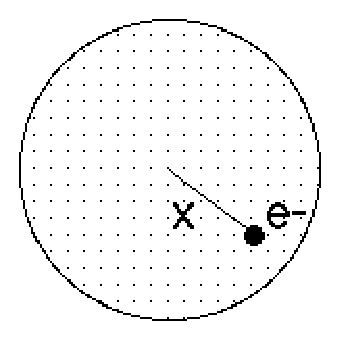
\includegraphics[clip,width=4cm]{AtomIdea/1-2.eps}
\caption{氢原子的汤姆逊模型}
\end{center}
\end{figure}

{\bf 例4 氢原子的汤姆逊模型}

考虑系统的稳定性,假设电子偏离平衡位置(球心)$x$,氢原子半径$a$,根据高斯定理,仅半径$x$球体内正电荷会与电子发生吸引。

\begin{equation}
F = m\ddot x =  - \left( {\frac{1}{{4\pi \varepsilon _0 x^2 }}}
\right)\left( {\frac{{x^3 }}{{a^3 }}} \right)e^2  =  - \left(
{\frac{1}{{4\pi \varepsilon _0 }}} \right)\left( {\frac{{e^2
}}{{a^3 }}} \right)x
\end{equation}

微分方程:$\ddot x + \omega ^2 x = 0$,频率为:$\omega  = \sqrt
{\frac{{e^2 }}{{4\pi \varepsilon _0 a^3 m}}} $,计算可得:$\nu =
\frac{\omega }{{2\pi }} = 2.5 \times 10^{15} Hz,\lambda  =
1200\mathop A\limits^o $
与氢原子光谱赖曼系第一支(Lyman-$\alpha$)吻合,但该模型无法解释氢原子其他的谱线。

\begin{figure}[h]
\begin{center}
  % Requires \usepackage{graphicx}
  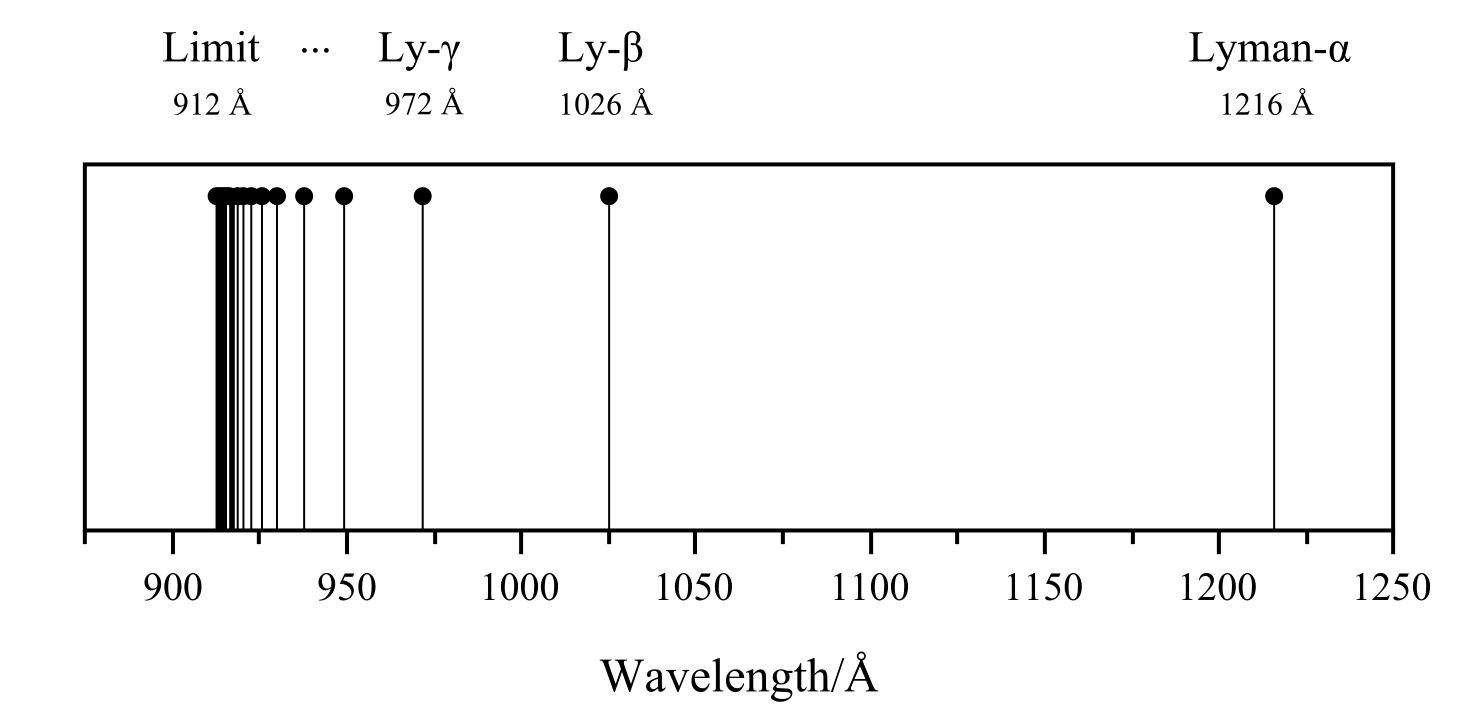
\includegraphics[width=10cm]{AtomIdea/LymanSeries.png}\\
  \caption{氢原子光谱赖曼系}\label{Lyman Series for Hydrogen atom}
\end{center}
\end{figure}



\subsection*{物理常数}

\begin{itemize}
  \item 阿佛加德罗常数: $N_A= 6.022 \times 10^{23} mole^{-1}$
  \item 法拉第常数: $F=9.648 \times 10^4 C \cdot mole^{-1}$
  \item 电子电量: $e = 1.602 \times 10^{-19} C$
  \item 电子质量: $m_e =9.109 \times 10^{-31}kg$
  \item 质子质量: $m_p = 1.673 \times 10^{27} kg$
  \item 光速:$c = 2.998 \times 10^8 m \cdot s^{-1}$
\end{itemize}

\subsection*{单位换算}

在粒子物理中, 我们通常用兆电子伏($MeV = 10^6 eV $)来表示粒子的质量.
请将电子质量($m_e$), 质子质量($m_p$)换算为$MeV$.

解: 根据相对论质能关系: $E=m_0 c^2$, 这里$m_0$是静止质量.
对电子而言,

\begin{equation*}
E = 9.109 \times 10^{-31} (3.0 \times 10^8)^2 = 8.2 \times 10^{-14}
J
\end{equation*}

相当于:

\begin{equation*}
\frac{8.2 \times 10^{-14}}{1.602 \times 10^{-19}} = 5.1 \times 10^5
eV = 0.51 \text{MeV}
\end{equation*}

假设质子“静能量”为$x$MeV,

\begin{equation*}
\frac{m_e c^2}{M_p c^2}=\frac{0.51}{x}
\end{equation*}

解出:

\begin{equation*}
x = 0.51 \cdot \frac{M_p}{m_e} =0.51 \times 1822 = 932
\end{equation*}

即质子“静能量”为932MeV, 或约1GeV.

\subsection*{阅读材料}


\begin{itemize}

  \item 原子的核心含义是“不可再分”,或按亚里士多德的“修正”,是某个层次(或技术条件)下的“不可再分”。我们有电的原子——电子,光的原子——光子,物质的原子——往往是分子(保持物质化学性质的最小单位)……

回到原子的本意——“不可再分”,原子在今天科学知识下的对应应是基本粒子(Elementary Particles),电子和光子都是基本的(不可再分的),原子核不是,它可以分为质子和中子,统称为重子(Baryons),重子也不是基本的,它由夸克组成,而夸克是基本的。

相关知识,请进一步阅读维基百科:Elementary particle

\url{http://en.wikipedia.org/wiki/Elementary_particle}

\item 原子物理标准的英文教材: B H Brandsden and C. J. Joachain, Physics of atoms and
  molecules. 
  
\item 阅读新科学家(New Scientist)文章: ``Roundest objects in the world
created'' \url{http://sinaurl.cn/7xVw3}

阿佛加德罗计划:如何通过完美的硅晶球精确定义千克(kg,国际单位制中的质量单位)。

\url{http://www.acpo.csiro.au/avogadro.htm}

\item 斯蒂芬·温伯格,《亚原子粒子的发现》
  
\item M Veltman, 《神奇的粒子世界》
  
\end{itemize}
